\chapter{问题描述}
\section{多目标检测与追踪问题描述}

给定图像序列${I_1, I_2,..., I_t}$, 每帧图像中有$M_t$个目标,其中t是当前帧号,每个目标的状态为$ s_1(t) $,其中状态一般包括位置,速度,加速度,朝向等。
\begin{equation}
	s_i(t) = \{ x,y,z,h,w,l,v_x,v_y,v_z,\theta \}
\end{equation}

当前帧的所有目标的状态就能表示成
\begin{equation}
	S(t) = \{ s_1(t), s_2(t),s_3(t),...,s_{M_t}(t) \}
\end{equation}

而每个目标的的轨迹则可以描述成
\begin{equation}
	s_i(1:t) = \{ s_i(1),s_i(2),s_i(3),...,s_i(t) \}
\end{equation}

则所有目标的状态集合就能表示成
\begin{equation}
	S(1:t) = \{ S_1. S_2,...S_t \}
\end{equation}

同理,我们类似的得到观测结果的定义,记作$ o_i(t),o_i(1:t),O(1:t) $。

而多目标跟踪任务就是通过观测结果找出所有目标的状态,我们用后验估计来进行描述。
\begin{equation}
	S(1:t) = argmax_{S(1:t)}P(S(1:t)|O(1:t))
\end{equation}

\section{问题的求解}
多目标检测与追踪一般的求解都基于TBD架构,如图\ref{dbt}所示。
\begin{figure}[H]
	\centering
	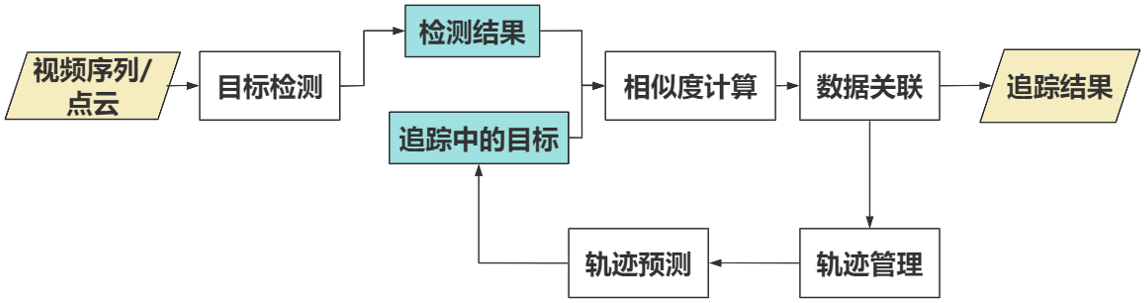
\includegraphics[width=\textwidth]{images/DBT.png}
	\caption{基于检测的追踪框架}
	\label{dbt}
\end{figure}


\section{滤波的作用}
主要概括,滤波的作用主要包括两个部分,融合多个传感器的追踪结果以及对目标进行预测,最终的目的都是为了得到更好的估计值。
它主要应用在图\ref{dbt}中轨迹预测部分。

\begin{tcolorbox}[]
	首先构建线性系统的状态空间描述:
	$$ \mathbf{x}_{t} = \mathbf{A} \mathbf{x}_{t-1} + \mathbf{B} \mathbf{u}_{t} + \bm{\epsilon}_{t} $$
	$$  \mathbf{z}_{t} = \mathbf{H} \mathbf{x}_{t} + \bm{\delta}_{t} $$
	
	接着利用卡尔曼滤波器进行最优状态估计:
	\begin{equation}
		\hat{\bm{x}}_{t}^{-} =  \bm{A} \hat{\bm{x}}_{t} + \bm{B} \bm{u}_t
	\end{equation}
	\begin{equation}
		\bm{\Sigma}_{t}^{-} = \bm{A} \bm{P}_{t-1} \bm{A}^{T} + \bm{Q}
	\end{equation}
	\begin{equation}
		\bm{K}_t = \frac{\bm{\Sigma}_{t}^{-} \bm{H}^{T}}{\bm{H} \bm{P}_{t}^{-} \bm{H}^{T} + \bm{R} }
	\end{equation}
	\begin{equation}
		\hat{\bm{x}}_t = \hat{\bm{x}}_{t-1} + \bm{K}_t(\bm{z}_t - \bm{H} \hat{\bm{x}}^{-})
	\end{equation}
	\begin{equation}
		\bm{P}_t = (\bm{I} - \bm{K}_t \bm{H}) \bm{P}_{t}^{-}
	\end{equation}
	
\end{tcolorbox}

\section{发展和思考}
1. \textbf{发展}

想要提高追踪的效果(精度,速度),可以从多个角度进行提高。大致可以包括几个方面:

仍旧基于BDT框架:追踪器的提升,数据融合方法的提升,数据关联的提升,滤波器的提升(包括模型改进)。

新的框架:端到端\cite{10610979},基于点的移动的追踪\cite{wu2024moving}。

2. \textbf{思考}

首先确定融合的框架:DBT和神经网络融合结构。
接着确定数据关联方式,倾向于用特征值(点)
然后改进滤波器的结构:模型的改进(长时间拟合),噪声的优化(A-KIT)
最后,连接最新的检测器。

实际实验:标定,ROS表示

\section{工作总结}
时间:11.18-11.24

工作内容:
对研究问题进行了数学上的描述;
学习了DFR-FastMOT和ByteTrack两篇文章,它们均对遮挡情况提出了不同解决方法;

工作展望:
将BYTE的思想移植到之前的追踪器中,看看提升的效果。
